\section{习题一 \ 舍入误差 $\epsilon$ }
\begin{enumerate}
    \item 最终计算得到的$f(x)$结果为0。出现该结果是由于在计算过程中,计算机位数长度的限制。$10^{-16}+1$在计算机内四舍五入为1,再减$1$变为0。
    \item \begin{python}
              for n in range(101, 0, -1):
              if (0.5 + 2 ** (-n)) > 0.5:
              print(n)
              break
          \end{python}
          最终输出结果为$n=53$。
\end{enumerate}

\section{习题二 \ 逼近指数函数}
\begin{figure}[htbp]
    \centering
    \subfigure[$x=10$]
    {
        \begin{minipage}[b]{.4\linewidth}
            \centering
            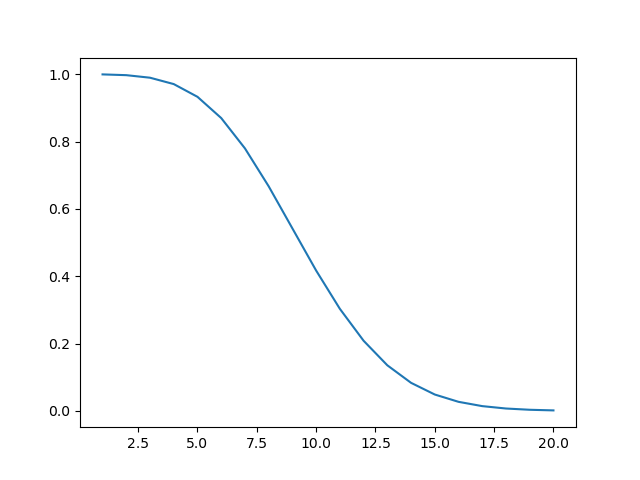
\includegraphics[scale=0.29]{pic/x=10.png}
        \end{minipage}
    }
    \subfigure[$x=-10$]
    {
        \begin{minipage}[b]{.4\linewidth}
            \centering
            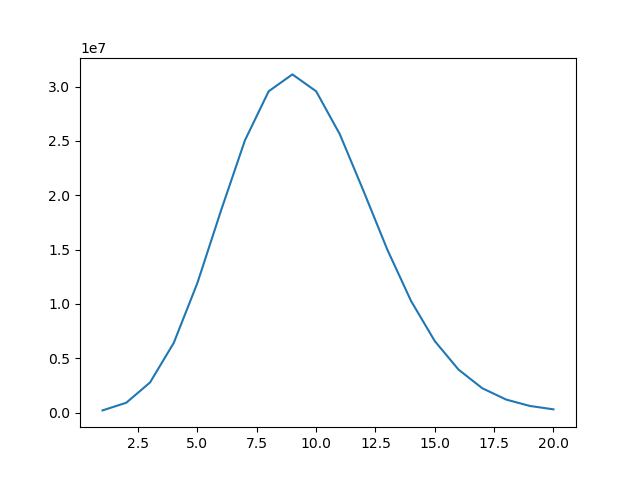
\includegraphics[scale=0.29]{pic/x=-10.png}
        \end{minipage}
    }
    \caption{相对误差}
\end{figure}
\begin{enumerate}
    \item $x=10$时相对误差逐渐下降,到$N=20$之后误差趋于稳定。
    \item $x=-10$时相对误差出现了波峰,直到$N=20$之后误差才趋于稳定,说明此逼近算法不够稳定。
    \item 可以采用插值算法对函数进行逼近。
\end{enumerate}

\section{习题三 \ 计算积分}
利用分部积分,可以得到
\begin{align}
    I_n & = \left[\left.xe^x\right|^{1}_{0} - \int^{1}_{0}nx^{n-1}e^xdx \right] \\
        & = \left[e^1 - n\int^{1}_{0}x^{n-1}e^xdx\right] \notag                 \\
        & = e-nI_{n-1} \notag
\end{align}
此即为递推公式。

以$I_0=e-1$为初始值,由递推公式可得$I_{20}=-129.26370813285942$。

